\documentclass[twoside,openright,a4paper,11pt,french]{article}
\usepackage[utf8]{inputenc}
\usepackage[french]{babel}
\usepackage[T1]{fontenc}
\usepackage{emptypage}

% Utilisation d'url
\usepackage{url}
\urlstyle{sf}

% Utilisation d'images, stockées dans le répertoire ./pics/
\usepackage{graphicx}
\graphicspath{pics/}

% Définition des marges
\usepackage{geometry}
\geometry{
  left=25mm,
  right=25mm,
  top=25mm,
  bottom=25mm,
  foot=15mm
}

\begin{document}

\pagestyle{plain}

% La page de garde
\thispagestyle{empty}

\begin{center}
       \noindent
       
\includegraphics[height=2.5cm]{./pics/uds.eps}       
       
       \vfill\vfill

    {\large \textsc{Licence 3 de Sciences, mention Informatique}}

    \bigskip\bigskip

    {\large \textsc{Réseaux et Protocoles}}

    \vfill\vfill

% Titre du document
    {\huge \sc
      \begin{center}
		Modèle de document\\pour un rapport d'étude
      \end{center}}

    \vfill\vfill

    {\large Présenté par}

\medskip

% Identité des auteurs
    {\large Julien \textsc{Montavont}}

% Contact mail
    {\small \url{montavont@unistra.fr}}

\bigskip

\end{center}



% La table des matières
\parskip=0pt
\tableofcontents


\section{Introduction}
\label{sec:intro}


\section{Concepts et utilisation}

% Luigi Coniglio 
\subsection{En-tete IPv4}
Un packet IPv4 est precede` par un en-tete ayant une longeur minimale de 20 octets 
(dans les cas aucune option supplementaire a ete specifie`).
La figure suivante montre le contenu de l'en-tete d'un packet IPv4.


% TODO FIGURE sans field options 
TODO FIGURE


Comme on peut voir dans la figure ci dessus, un en-tete IPv4 est compose` par
13 champs. En realite nous verrons plus loin que cet en-tete peut, quand il est
necessaire, contenir un champ additionel qui servira a specifier quelque
option qui n'est pas presente dans le 13 champs ci dessus.


Commencons par voir plus en detail les 13 champs d'un en-tete IPv4 standard:

\begin{description}
\item [Version] 
Cette champ occupe les premiers 4 bits de l'en-tete IPv4. Il est
utilise pour determiner le type de protocole utilise` par la couche
reseau (chouche 3). Dans le cas de IPv4 cet champs contiendra toujours
la valeur 4, qui justement identifie le protocole IPv4.

Cet champ n'est pas tres utilise, en tenant compte que le protocole 
a utiliser pour la couche 3 est presque toujour specifie dans l'en-tete
de la couche liason.

\item [IHL]
Le champ IHL specifie la taille de l'en-tete IPv4, en fait IHL est 
l'acronime de Interet Header Length. Bien entendu, en disant cela on souligne
un concept important a propos du protocole IPv4: la taille de l'en-tete n'est pas fixe.

La taille de l'en-tete est exprime`e en bloques de 32 bits. Etant donne une taille de
4 bits pour le champ IHL, la longueur maximale d'un en-tete IPv4 est de 15 bloques de
32 bits, qui correspond a 60 octets. Comme l'en-tete IPv4 a une taille minimale
de 20 octets (160 bits), le champ IHL ne peut pas contenir un valeur inferieure a 5.

\item [Type of Service]
Le champ Type of Service, mieux connu avec l'acronime ToS, est utilise pour 
specifier la qualite de service souhaite pour l'envoi d'un packet IPv4.
Cet champ occupe un octet de l'en-tete et il se compose en trois parties.
Une premiere partie de 3 bits permet d'indiquer la precedence avec la quelle
le packet doit etre traite, les 3 bits apres sont utilise pour specifier 
certaines caracteristiques du service, notament: le temp, le debit et la fiabilite.
Enfin l'emploi des 2 derniers bits n'a pas ete specifie et leur usage a ete 
laisse libre pour des implementationes futures.


En realite l'histoire de cet champs est bien plus longue et complexe que ca,
car en pratique la facon d'utiliser cet champs a ete modifie plusieurs fois au 
cours des annees.
\footnote{L'utilisation des 8 bits du champ ToS a ete redefinie
par cinq standard differents (plus divers standars experimentals).
Les documents presentent ces standard sont mentionne dans le chapitre 
"Historical Definitions for the IPv4 TOS Octet" du RFC 3168}
Cette manque de stabilite a par fois cause une certaine confusion dans les implementations.
\footnote{Comme le souligne le RFC 3260 {\it "At least one implementor has expressed confusion about the
relationship of the DSField, as defined in RFC 2474, to the use of
the TOS bits, as described in RFC 1349"}}

Aujourd'hui les 8 bits du champ ToS sont utilise par le mecanisme DiffServ
(Differentiated Services). Cet systeme utilise les premieres 6 bits du champ
ToS (DSCP - Differentiated Services Code Point) pour marquer chaque paquet
comme appartenant a un niveau de priorite et une classe de service.  Chaque
classe determine le type de traitement que on souhaite demander pour le paquet
aux routers au long du chemin (PHB - Per-Hop behaviour), toutefois le service offert
par chaque router est fortement lie a sa configuration.
\footnote {
{\it "The DiffServ standard does not specify a precise definition of "low," "medium,"
and "high" drop probability. Not all devices recognize the DiffServ (DS2 and
DS1) settings; and even when these settings are recognized, they do not
necessarily trigger the same PHB forwarding action at each network node. Each
node implements its own response based on how it is configured."} - 
Implementing Quality of Service Policies with DSCP
http://www.cisco.com/c/en/us/support/docs/quality-of-service-qos/qos-packet-marking/10103-dscpvalues.html
}}
Le dernieres 2 bits du champ ToS sont utilise pour l'extension ECN ({\it Explicit Congestion
Notification }). Cette extension, propose par RFC2481 et introduite deux annees apres avec le RFC3168,
ajoute un systeme de controle de la congestion du traffic reseau. Dans le cas d'une saturation
de la reseau cet champ est utilise pour notifier cet probleme et demander a le dispositif emetteur
une reduction du rythme au quel les packets sont envoye, avec l'objectif de reduir l'attente et
la perte de packets.

\item [Total length]
Comme le suggere le nom, ce champs est utilise pour indiquer la taille totale du
packet IPv4: en tete plus donnes. Le champ {\it Total length} est defini sur 16
bits, ceci permet de indiquer un valeur compri entre 0 et 65,535 octets. Comme l'en-tete
est compris dans la longeur totale d'un packet cet valeur ne sarait jamais inferieur
a 20 (taille minimale d'un en-tete IPv4 en octets).
RFC 791 impose a toutes les dispositifs d'une reseau IPv4 la capacite de recevoir
des packets jusq'a une taille de 576 octets, cette prerogative permet de
eviter une excessive fragmentation.

\item [Identification]
Cet en-tete (sur 16 bits) permet d'identifier les fragments appartenent au meme packet.

\item [Flags]
Le 3 bits du champs Flags sont utilise pour gerer la fragmentation d'un packet.
Un de ces bit est emploie pour indiquer si le paquet peut etre fragmente ou
non. Cet bit, appelle DF ({\it Don't Fragment}), doit etre pris en consideration
par les routers dans le chemin pour decider si un paquet trop grand pour etre
trasmis peut etre retrasmis sous forme de fragments plus petits ou rejete. 
Un autre bit, appelle MF ({\it More Fragments}), indique si le paquet est suivi 
par d'autres fragments. Le bit MF est mis a 0 dans le dernier fragment ou dans
des paquet qui n'ont pas ete fragmente.

Un des trois bits de ce champs n'est pas actuallement utilise mais il a ete
reserve pour applications futures possibles.
\footnote {Cet bit a ete aussi le protagoniste d'un des plus connu poissons
d'avril presentee par le IETF. Pour faciliter les taches des systems de filtrage 
le RFC 3514 propose d'utiliser ce bit pour etiqueter paquets mailveillant, a ce
titre tous les paquets etant envoye avec ce bit (renomme "{\it Evil Bit}") 
mis a 1 seront mis a la poubelle.
}

\item [Fragment Offset]
Lorsque un paquet a ete fragmentee cet en-tete est utilisee pour determiner la 
position (offset) d'un fragment par rapport a les donnees du paquet reassemble.
Le decalage de chaque fragment est exprime en bloques de huit octets (ou 64
bits).  Le champ Fragment Offset utilise 13 bits de l'en-tete IPv4, cela permet
un offset maximale de 65,528 octets.\footnote {En pratique un tel offset n'est
jamais utilisee car, en ajoutant un en-tete minimale de 20 octets, la taille 
totale du paquet reassemble depaserait la longeur maximale d'un paquet IPv4.}
Etant donne que la flag MF ({\it More Fragments}) doit etre mise a zero lorsque 
si un paquet n'est pas fragmentee ou si il est le dernier fragment d'un paquet
plus grand, l'unique difference entre ce deux types de paquets est le valeur
de le champ Fragement Offset que, dans le cas d'un paquet pas fragmentee, est
toujours zero.

\end{description}




\section{Suite de protocole}

\subsection{ARP}
ARP (Address resolution protocol) est un protocole à cheval sur la couche 2 et
la couche 3. La fonction principale d'ARP est de faire la conversion entre les
adresses de niveau 2 et de niveau 3. Cela est très utilisé étant donné que les
hôte connaissent souvent les adresses IP de leur destinataire, mais rarement
l'adresse de niveau 2 de ce destinataire ou de la passerelle à contacter pour joindre
le destinataire.

\subsubsection{Exemple}
Dans la partie qui suit nous allons nous placer dans l'exemple suivant.
TODO LAN exemple
\subsubsection{Entête}

\subsubsection{Fonctionnement}
Prenons l'exemple où A veux envoyer un message à B. A connait l'adresse IP de
B. Donc A va préparer son paquet qu'il va envoyer à B, avec son adresse IP en
source et l'adresse IP de B en destination. La paquet passe dans la couche
liaison, il va être enpaqueté dans une trame de niveau 2. Cette trame aura
comme adresse source l'adresse de niveau 2 de A, mais à ce moment il ne peux
pas completé l'adresse destination de la trame: en effet, il ne connait
l'adresse de niveau 2 du destinataire. La paquet reste bloqué en couche 2 et ne
peux pas être envoyé au destinataire. Comment obtenir l'adresse de niveau 2 du destinaire?
Le protocole ARP est capable de faire cette translation.

\subsubsection{ACD}
Adresse conflict detection
\subsection{ICMP}
ICMP (Internet Control Message Protocol) est un protocole de niveau 3 faisant partie intégrante du protocole IPv4. Il permet de transmettre des informations de controle et d'erreur. Les messages ICMP sont empaquetés dans des paquets IP, ils diposent donc d'un entête de paquet IP. Cet entête est le même que pour tout les autres entêtes de paquet d'IPv4. Deux champs son intéressant dans le cas d'un paquet ICMP, les champs Protocol et Type of service. Le champ Protocol est mis à à la valeur 1 pour dire que le paquet contient un message ICMP, et le champ ToS est mis à 0 //TODO(pourquoi 0?)//.
Après le header du paquet IPv4, commence la partie data qui contient le message ICMP. Ce message contient des champs différent en fonction du type de message à passer. Cependant les trois premier champs sont toujours les mêmes.
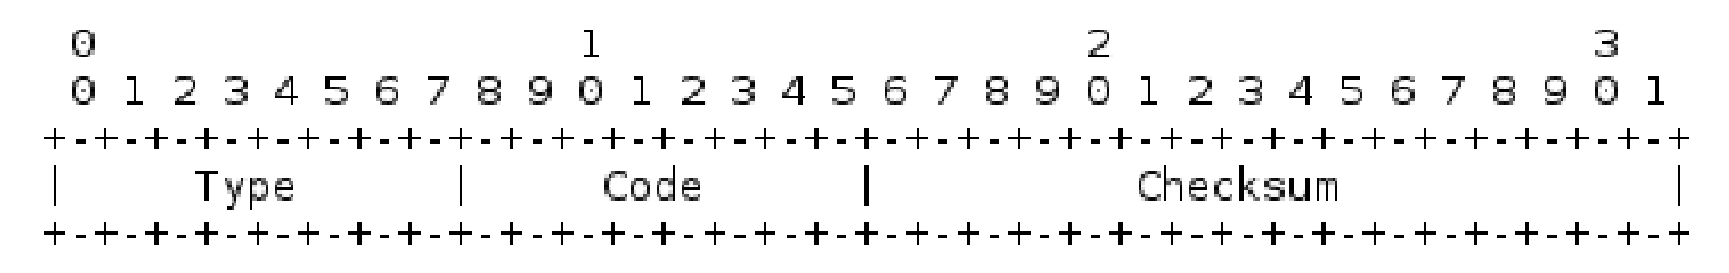
\includegraphics[width=15cm]{./pics/header.eps}
\\Le premier champ est celui de type. Il permet, premièrement, de donner le type du paquet et de l'information à transmettre, et deuxièmement de préciser la nature des champs qui vont suivres. En effet, comme vu plus haut, les messages contiennent des champs différents selon le type du message ICMP.
\\Le deuxième champ est le code. Il permet de subdiviser le type en donnant des détails plus précis.
\\Enfin le troisième champ est la somme de contrôle (checksum)//TODO(plage de controle).
\\Commençons avec les messages qui possèdent l'ensemble de champs le plus simple.

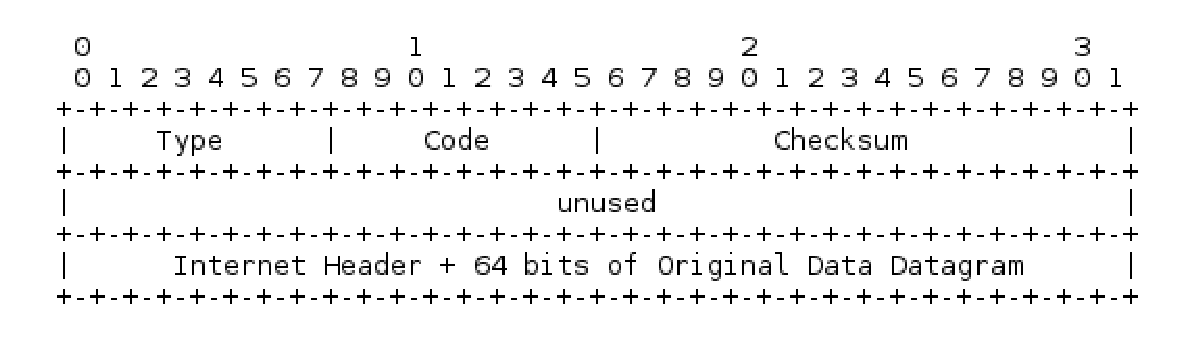
\includegraphics[width=15cm]{./pics/header1.eps}

\\Les messages qui utilisent cette organisation sont les messages de type 3, 4 et 11.

\subsubsection{Message de type 3: Unreachable Destination}
Les messages de type 3 sont émis lorsqu'un paquet n'a pas réussi à joindre la destination (Unreachable destination). Cette erreur peux être dut à plusieurs facteurs, et les codes permettent de préciser pourquoi le paquet n'a pas pu rejoindre sa destination.
\paragraph{Code 0}

\subsubsection{Message de type 4:}
\subsubsection{Message de type 11: Time Exceeded}
Ces messages sont envoyés lorsque le TTL d'un paquet à atteind 0. Une autre utilisation des ces messages est lorsque que le temps de ré-assemblage des fragments d'un paquet est dépassé. Ces deux cas sont distingé par le code. Ces messages ont pour destinataire l'hôte qui à envoyé le paquet qui à provoqué l'erreur.//TODO(vérifier)
\paragraph{Code 0}
Le code 0 est utilisé pour indiquer que le TTL du paquet posant problème est arrivé à 0. Lorsque le TTL d'un paquet arrive à 0, celui-ci est supprimer et un message ICMP de type 11 et de code 0 est envoyer par le routeur qui à détécté le problème. Cela permet principalement d'éviter qu'un paquet sans dans une boucle et qu'il soit rélayé à l'infini.
\paragraph{Code 1}
Le code 1 est quant à lui utilisé pour indiquer //TODO
\subsection{IGMP}
\subsection{DHCP}







\section{Conclusion}
\label{sec:ccl}

\cleardoublepage
\addcontentsline{toc}{section}{Références}
\bibliographystyle{plain}
\bibliography{rapport}

\end{document}
